\documentclass{article}

\usepackage[most]{tcolorbox}
\usepackage{physics}
\usepackage{graphicx}
\usepackage{float}
\usepackage{amsmath}
\usepackage{amssymb}


\usepackage[utf8]{inputenc}
\usepackage[a4paper, margin=1in]{geometry} % Controla los márgenes
\usepackage{titling}

\title{Clase 6}
\author{Manuel Garcia.}
\date{\today}

\renewcommand{\maketitlehooka}{%
  \centering
  \vspace*{0.05cm} % Espacio vertical antes del título
}

\renewcommand{\maketitlehookd}{%
  \vspace*{2cm} % Espacio vertical después de la fecha
}

\newcommand{\caja}[3]{%
  \begin{tcolorbox}[colback=#1!5!white,colframe=#1!25!black,title=#2]
    #3
  \end{tcolorbox}%
}

\begin{document}
\maketitle

\caja{blue}{Parametrizacion cinta de moebius }{
  Hacer ejercicio del taller 2 de la cinta de moebius.
}
\section{ejercicio 17 taller 1 (Pregunta raisuke)}
\begin{gather}
  \frac{\bra{\dot r }\ket{[\ddot r, \dddot r ]} }{\left|[\dot r, \dot r ]\right|} = - \chi 
\end{gather}
Tenemos que: 
\begin{gather}
  \dot r = \frac{d r  }{d l }\frac{1}{v_t } = \frac{v }{\left|v_z \right|}\\    
  \ddot  = \frac{d}{dt }\left(\frac{d r }{d l} \frac{1}{v_t }\right) = ... f v + \beta n \\
  \dddot r = \alpha v + \beta n + \nu b 
\end{gather}

\caja{black}{Parametrizado en terminos de la longitud de arco }{
  Si la norma de la velocidad en terminos del tiempo es igual a 1 entonces está parametrizado en terminos de la longitud de arco $ \left|v_t \right| = \frac{d l  }{d t} =1 $
}

\section{Segunda forma fundamental en una superficie}
Entorno a un punto regular $ P_0  = (x_0,y_0,z_0) $ se puede describir una superficie por medio de $ z = f\left(x,y\right) $ de tal manera que el eje z sea perpendicular a la superficie en ese punto. De esta forma $ \grad f = 0|_{P_0 } $, ya que la 1ra variación de la función es cero, a continuación se toma la segunda variación: 
\begin{gather}
  d ^ {2 }f = f _{xx } dx ^2 + 2 f _{xy } dx dy + f _{yy } dy ^ {2 }  
\end{gather}
Matrix Hessiana: 
\begin{gather}
  H _{ij }  = \begin{bmatrix}
      f _{xx }  & f _{xy }  \\
      f _{xy }  & f _{yy } 
  \end{bmatrix} . \qquad H _{ij } = H _{ji }   
\end{gather}

En una situación más general que la descrita antes, podemos usar una representación paramétrica de la superficie $ r\left(u,v\right)  $ y calcular la curvatura de una curva en la superficie. Para eso necesitamos calcular la aceleración de la curva: 
\begin{gather}
  r\left(u,v\right) \rightarrow \qquad \ddot r\left(u,v\right)=r _{uu } \dot u ^ {2 } + 2 r _{vu } \dot u \dot v + r _{vv } \dot v ^ {2 } + r _{u } \ddot u + r _{v } \ddot v 
\end{gather}
A continuación proyectamos la aceleración sobre el vector normal unitario a la superficie $ N = \frac{[r _{u } , r _{v } ]}{|[r _{u } , r _{v } ]|} $   
\begin{gather}
  \bra{\ddot r }\ket{N } = \bra{r _{uu }}\ket{N }\dot u ^ {2 } + 2 \bra{r _{vu } }\ket{N }\dot u \dot v + \bra{r _{vv } }\ket{N }\dot v ^ {2 }\\
  \bra{\ddot r }\ket{N }dt ^2 = \bra{r _{uu } }\ket{N }du ^2 + 2 \bra{r _{vu } }\ket{N }du dv + \bra{r _{vv } }\ket{N }dv ^2 = b _{ij } dx ^ {i }dx ^ {j }    
\end{gather}
\caja{green}{Segunda forma fundamental en la superficie }{
  La proyección de la aceleración sobre la noral es una forma cuadrática para vectores angentes a la superficie. esta forma cuadrática es la segunda forma fundamental en la superficie. 
  \begin{gather}
    \bra{\ddot r }\ket{N }dt ^ {2 } = L du ^ {2 } + 2M du dv + \bar N dv ^ {2 } = b _{ij } dx ^ {i }dx ^ {j }  
  \end{gather}
}

\textbf{Procedimiento }

Tenemos que $ \ddot r (u,v) \rightarrow \ddot r = \frac{d  }{d t}\left[r _{u } \dot u + r _{v } \dot v \right] $, entonces: 
\begin{gather}
  \ddot r = (r _{uu } \dot u + r _{uv } \dot v )\dot u + r _{u } \ddot u + ( r _{vu } \dot u + r _{vv } \dot v )\dot v + r _{v } \ddot v \\
  = r _{uu} \dot u ^ {2 } + 2 r _{uv } \dot u \dot v + r _{vv } \dot v ^ {2 } + ( r _{u } \ddot u + r _{v } \ddot v )
\end{gather}
Podemos hacer: 
\begin{gather}
  \bra{\ddot r }\ket{N } = \bra{r _{uu } }\ket{N }\dot u ^ {2 } + 2 \bra{r _{uv } }\ket{N }\dot u \dot v + \bra{r _{vv } }\ket{N }\dot v ^ {2 }\\
  N \equiv \frac{[r _{u } , r _{v } ]}{\left|[r _{u } , r _{v } ]\right|}\\
  \bra{\ddot r }\ket{N }dt ^ {2 } = \bra{r _{uu} }\ket{N }du ^ {2 } + 2 \bra{r _{uv } }\ket{N }dudv + \bra{r _{vv } }\ket{N } dv ^ {2 }\\
  \bra{\ddot r }\ket{N }dt ^ {2 } = b _{ij } dx ^ {i }dx ^ {j } = L du ^ {2 } + 2 M dudv + \bar N dv ^ {2 }\\
  b _{ij }  = \begin{bmatrix}
      L & M \\
      M & \bar N 
  \end{bmatrix}  
\end{gather}
Por lo tanto podemos hacer: 
\begin{gather}
  \bra{\ddot r }\ket{N }dt ^ {2 } = b _{ij } dx ^ {i }dx ^ {j } \qquad \qquad t = s \\
  \bra{\ddot r }\ket{N }ds ^ {2 } = \bra{\dot r }\ket{N } g _{ij } dx ^ {i }dx ^ {j } = b _{ij } = b _{ij } dx ^ {i }dx ^ {j }\\
  \bra{\ddot r }\ket{N } = \frac{b _{ij } dx ^ {i }dx ^ {j }}{g _{ij } dx ^ {i }dx ^ {j }} = b _{ij } \frac{\dot x ^ {i }\dot x ^ {j }}{g _{ij } \dot x ^ {i }\dot x ^ {j }} 
\end{gather}
Utilizando las formas de fernet serrat: 
\begin{gather}
  \bra{\ddot r }\ket{N } = \bra{kn }\ket{N } = k \bra{n}\ket{N} = k \cos{\theta} = k _{n } \quad \text{k normal}
\end{gather}
\begin{figure}[H]
  \begin{center}
    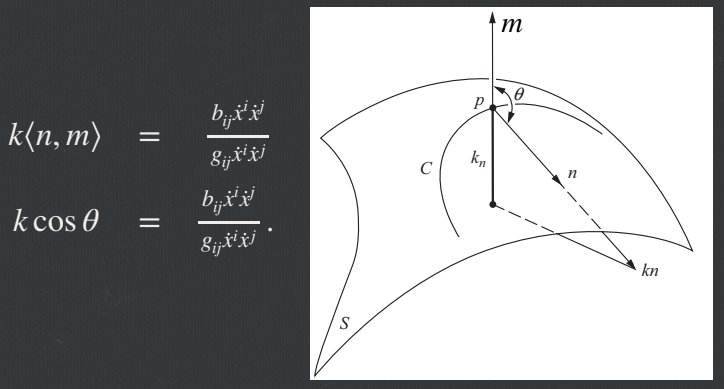
\includegraphics[width=0.5\textwidth]{knormal.png}
  \end{center}
\end{figure}

\section{Mapeo de gauss }
\textbf{Orientacion de una superficie }: 
\begin{gather}
  N = \frac{[r _{u } , r _{v } ]}{\left|[r _{u } , r _{v } ]\right|} 
\end{gather}
\caja{green}{Mapeo de gauss }{
  \begin{gather}
    N : S \rightarrow S ^ {2 }\\
    S ^ {2 } = \{ (x,y,z) \in \mathbb{R}; x ^ {2 } + y ^ {2 }+ z ^2 = 1   \}
  \end{gather}
  \textbf{Diferencial del mapeo de Gauss }
  \begin{gather}
    dN _{p } : T _{p } (S) \rightarrow T _{p } (S ^ {2 })\\
    T _{p } = T _{p } (S ^ {2 })\\
    \rightarrow dN _{p } : T _{p } (S) \rightarrow T _{p } (S)
  \end{gather}
  $ d N _{p }  $ está en $ T _{p } (S)  $. Notar que: 
  \begin{gather}
    \bra{N}\ket{N} = 1 \rightarrow \bra{dN }\ket{N } = 0 \rightarrow dN _{p } \in T _{p } (S)   
  \end{gather}
  \tcblower 
  El mapeo de gauss es diferenciable y lineal.
}
\begin{figure}[H]
  \begin{center}
    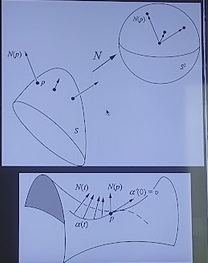
\includegraphics[width=0.4\textwidth]{mapeo_gauss.png }
  \end{center}
\end{figure}

\textbf{Ejemplos }

\textbf{Plano }
\begin{gather}
  ax + by + cz + d = 0, \qquad N = \frac{(a,b,c) }{(a ^2 + b ^2+ c ^2 )^ {1/2 }}\\
  N (\alpha(t)) = N \qquad const. \rightarrow dN = 0
\end{gather}
A esto se llega de la siguiente forma: 
\begin{gather}
  \vec N . \Delta \vec r = 0 \\   
  a \Delta x + b \Delta y + x \Delta z  = 0 \\
  ax+by+cz+d = 0
\end{gather}

\textbf{Esfera }
\begin{gather}
  S ^2 = \{ (x,y,z) \in \mathbb{R}^ {3 }; x ^2+ y ^2+ z ^2 = 1  \} \\
  \alpha(t) = (x\left(t\right), y\left(t\right), z\left(t\right)), \quad \rightarrow \quad 2x x' + 2yy' + 2zz'  = 0 \\
  N(t)= - (x\left(t\right), y\left(t\right), z\left(t\right)), dN(t) = - (x'\left(t\right), y'\left(t\right), z'\left(t\right))\\
  dN _{p } (v) = -v 
\end{gather}
A se llega d ela siguiente forma: 
\begin{gather}
  x ^2(t) + y ^2(t)+ z ^2(t) = 1 \quad \rightarrow \quad 2x \frac{d x }{d t} + 2y \frac{d y }{d t} + 2z \frac{d z }{d t} = 0 \\
  \underset{\dot \alpha(t)}{(-\dot x , - \dot y, - \dot z )}. \underset{N }{(-x,-y,-z)} = 0 \\
  N = \frac{- (x,y,z )}{(x ^2+ y ^2+ z ^2 )^ {1/2 }} \qquad \qquad \bra{dN }\ket{N } = 0 \\
  dN = -(\dot x, \dot y, \dot z )dt
\end{gather}

\subsection{Propiedad (autoadjunto)}
El diferencial del mapeo de Gauss $ dN _{p } : T _{p } (S)\rightarrow T _{p } (S) $ cumple la propiedad: 
\begin{gather}
  \bra{dN _{p } (w _{1 } )}\ket{w _{p } } = \bra{w _{1 } }\ket{dN _{p } (w _{p } )}, \qquad \forall (w_1,w_2) \in T _{p } (S)
\end{gather}
Donde $ w_1,w_2  $ son vectores tangentes a las curvas $ \alpha_1(t),\alpha_2(t) $ respectivamente. 

\hfill

\textbf{Prueba: }
Para la prueba recordemos que $ \bra{dN_p (w_1 )}\ket{w_2 } = \bra{w_1 }\ket{dN_p (w_2 )}   $.

primero escribamos de forma explicita el resutlado de evaluar un vector tangente $ w = \alpha'(0 ) $ en el mapeo $ dN _{p }  $. 
\begin{gather}
  dN_p (\alpha'(0)) = \frac{\partial N }{\partial u}\dot u + \frac{\partial N }{\partial v}\dot v |_{t=0 }  = N_u \dot u (0) + N_v \dot v(0)\\
\text{Aplicando esto en la primera eq que recordamos para la prueba: }\\
  \bra{N_u \dot u_1(0)+ N_v \dot v_1(0)}\ket{r_u \dot u _2 (0) + r_v \dot v_2 (0)} \\
  = \bra{N_u }\ket{r_u }\dot u_1(0) \dot u_2(0) + \bra{N_u }\ket{r_u }\dot u_1(0)\dot v_2(0)+ \bra{N_v }\ket{r_u }\dot v_1(0)\dot u _2 (0) + \bra{N_u }\ket{r_v }\dot v_1 (0)\dot v_2(0)\\
\end{gather}

Tambien tenemos que: 
\begin{gather}
  \bra{r_u \dot u _1 (0) + r_v \dot v_1 (0)}\ket{N_u \dot u _2(0) + N_v \dot v_2 (0)}\\
  = \bra{r_u }\ket{N_u }\dot u _1 (0) \dot u _2 (0) + \bra{r_u }\ket{N_v }\dot u_1 (0)\dot v_2 (0) + \bra{r_v }\ket{N_u }\dot v_1 (0)\dot u_2 (0) + \bra{r_v }\ket{N_v }\dot v_1(0) \dot v_2(0)    
\end{gather}

Por lo tanto: 
\begin{gather}
  \bra{r_u }\ket{N_v } = \bra{N_u }\ket{r_v }\\
  \bra{N}\ket{r_u } = \bra{N}\ket{r_v } = 0 \\
  \bra{N_v }\ket{r_u }+ \bra{N}\ket{r _{uv } }\\  
  \bra{N_v }\ket{r_u } = - \bra{N }\ket{r_uv }  
\end{gather}
y 
\begin{gather}
  \bra{N_u }\ket{r_v }+ \bra{N }\ket{r _{vu } }\\
  \bra{N_u }\ket{r_v } = - \bra{N }\ket{r _{vu } }  
\end{gather}

\caja{green}{Teorema de meusnier }{
  Todas las curvas obtenidas de cortar S con un plano (por ejemplo $ C  $y $ C_n  $), que comparten la misma tangente en un punto p, tienen la misma cudrvatura normal: 
  \begin{gather}
    k_n = \pm \frac{b _{ij }\dot x ^ {i }\dot x ^ {j }}{g _{ij }\dot x ^ {i }\dot x ^ {j }} \\
    k_n = \pm \frac{b _{ij }v ^ {i }v ^ {j }}{g _{ij }v ^ {i }v ^ {j }} 
    \label{eq:teo_meusnier}
  \end{gather}
}

No entendí bien qué se hizo a continuacion xd

\begin{gather}
  \bra{N }\ket{\alpha'(0)} = 0 \rightarrow \frac{d  }{d s} \rightarrow \left(\bra{\frac{d N }{d S }} \ket{\alpha'(S)} + \bra{N }\ket{\alpha''}  \right)|_{t = 0 }  = 0 \\
  \bra{\frac{d N }{d S}}\ket{v } + \bra{N }\ket{kn } = \text{algo }+ k \cos{\theta}\\
  \bra{\frac{d N  }{d S }}\ket{\alpha'(S) }| _{t = 0 } = - \bra{N }\ket{\alpha''(S)} = -k \cos{\theta}\\
  \bra{dN_p(v)}\ket{v} = - \Pi _p (v) = -k \cos{\theta}
\end{gather}
\caja{red}{}{
  \begin{gather}
    \Pi _p (v) = k \cos{\theta} = k_n  
  \end{gather}
}

\end{document}
